\documentclass{standalone}
\usepackage{tikz}
\begin{document}
% Created by tikzDevice version 0.7.0 on 2014-12-04 15:29:12
% !TEX encoding = UTF-8 Unicode
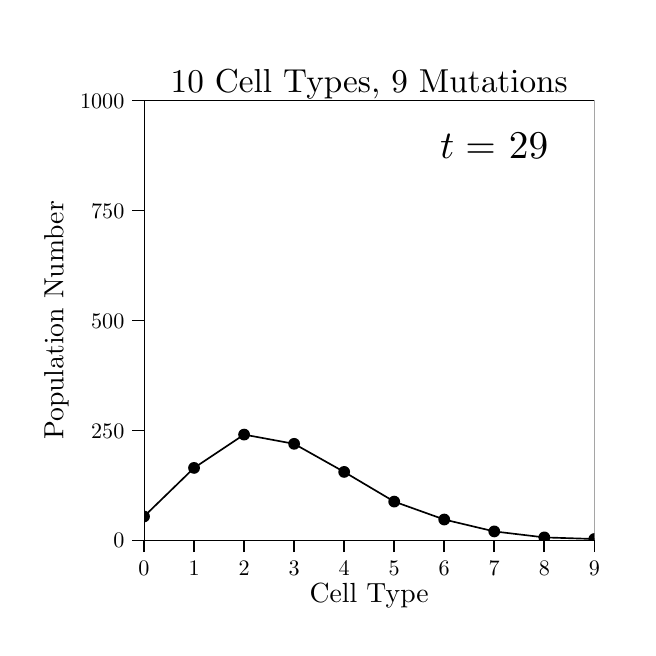
\begin{tikzpicture}[x=1pt,y=1pt]
\definecolor[named]{fillColor}{rgb}{1.00,1.00,1.00}
\path[use as bounding box,fill=fillColor,fill opacity=0.00] (0,0) rectangle (216.81,216.81);
\begin{scope}
\path[clip] (  0.00,  0.00) rectangle (216.81,216.81);
\definecolor[named]{drawColor}{rgb}{1.00,1.00,1.00}
\definecolor[named]{fillColor}{rgb}{1.00,1.00,1.00}

\path[draw=drawColor,line width= 0.6pt,line join=round,line cap=round,fill=fillColor] ( -0.00,  0.00) rectangle (216.81,216.81);
\end{scope}
\begin{scope}
\path[clip] ( 42.04, 31.56) rectangle (204.76,190.48);
\definecolor[named]{fillColor}{rgb}{1.00,1.00,1.00}

\path[fill=fillColor] ( 42.04, 31.56) rectangle (204.76,190.48);
\definecolor[named]{drawColor}{rgb}{0.00,0.00,0.00}

\path[draw=drawColor,line width= 0.6pt,line join=round] ( 42.04, 40.18) --
	( 60.12, 57.73) --
	( 78.20, 69.77) --
	( 96.28, 66.43) --
	(114.36, 56.28) --
	(132.44, 45.56) --
	(150.52, 39.08) --
	(168.60, 34.78) --
	(186.68, 32.62) --
	(204.76, 32.04);
\definecolor[named]{fillColor}{rgb}{0.00,0.00,0.00}

\path[fill=fillColor] ( 42.04, 40.18) circle (  2.13);

\path[fill=fillColor] ( 60.12, 57.73) circle (  2.13);

\path[fill=fillColor] ( 78.20, 69.77) circle (  2.13);

\path[fill=fillColor] ( 96.28, 66.43) circle (  2.13);

\path[fill=fillColor] (114.36, 56.28) circle (  2.13);

\path[fill=fillColor] (132.44, 45.56) circle (  2.13);

\path[fill=fillColor] (150.52, 39.08) circle (  2.13);

\path[fill=fillColor] (168.60, 34.78) circle (  2.13);

\path[fill=fillColor] (186.68, 32.62) circle (  2.13);

\path[fill=fillColor] (204.76, 32.04) circle (  2.13);

\node[text=drawColor,anchor=base,inner sep=0pt, outer sep=0pt, scale=  1.42] at (168.60,169.70) {$t = $ 29};

\path[draw=drawColor,line width= 0.6pt,line join=round,line cap=round] ( 42.04, 31.56) rectangle (204.76,190.48);
\end{scope}
\begin{scope}
\path[clip] (  0.00,  0.00) rectangle (216.81,216.81);
\definecolor[named]{drawColor}{rgb}{0.00,0.00,0.00}

\node[text=drawColor,anchor=base east,inner sep=0pt, outer sep=0pt, scale=  0.80] at ( 34.93, 28.80) {0};

\node[text=drawColor,anchor=base east,inner sep=0pt, outer sep=0pt, scale=  0.80] at ( 34.93, 68.53) {250};

\node[text=drawColor,anchor=base east,inner sep=0pt, outer sep=0pt, scale=  0.80] at ( 34.93,108.26) {500};

\node[text=drawColor,anchor=base east,inner sep=0pt, outer sep=0pt, scale=  0.80] at ( 34.93,147.99) {750};

\node[text=drawColor,anchor=base east,inner sep=0pt, outer sep=0pt, scale=  0.80] at ( 34.93,187.72) {1000};
\end{scope}
\begin{scope}
\path[clip] (  0.00,  0.00) rectangle (216.81,216.81);
\definecolor[named]{drawColor}{rgb}{0.00,0.00,0.00}

\path[draw=drawColor,line width= 0.6pt,line join=round] ( 37.77, 31.56) --
	( 42.04, 31.56);

\path[draw=drawColor,line width= 0.6pt,line join=round] ( 37.77, 71.29) --
	( 42.04, 71.29);

\path[draw=drawColor,line width= 0.6pt,line join=round] ( 37.77,111.02) --
	( 42.04,111.02);

\path[draw=drawColor,line width= 0.6pt,line join=round] ( 37.77,150.75) --
	( 42.04,150.75);

\path[draw=drawColor,line width= 0.6pt,line join=round] ( 37.77,190.48) --
	( 42.04,190.48);
\end{scope}
\begin{scope}
\path[clip] (  0.00,  0.00) rectangle (216.81,216.81);
\definecolor[named]{drawColor}{rgb}{0.00,0.00,0.00}

\path[draw=drawColor,line width= 0.6pt,line join=round] ( 42.04, 27.29) --
	( 42.04, 31.56);

\path[draw=drawColor,line width= 0.6pt,line join=round] ( 60.12, 27.29) --
	( 60.12, 31.56);

\path[draw=drawColor,line width= 0.6pt,line join=round] ( 78.20, 27.29) --
	( 78.20, 31.56);

\path[draw=drawColor,line width= 0.6pt,line join=round] ( 96.28, 27.29) --
	( 96.28, 31.56);

\path[draw=drawColor,line width= 0.6pt,line join=round] (114.36, 27.29) --
	(114.36, 31.56);

\path[draw=drawColor,line width= 0.6pt,line join=round] (132.44, 27.29) --
	(132.44, 31.56);

\path[draw=drawColor,line width= 0.6pt,line join=round] (150.52, 27.29) --
	(150.52, 31.56);

\path[draw=drawColor,line width= 0.6pt,line join=round] (168.60, 27.29) --
	(168.60, 31.56);

\path[draw=drawColor,line width= 0.6pt,line join=round] (186.68, 27.29) --
	(186.68, 31.56);

\path[draw=drawColor,line width= 0.6pt,line join=round] (204.76, 27.29) --
	(204.76, 31.56);
\end{scope}
\begin{scope}
\path[clip] (  0.00,  0.00) rectangle (216.81,216.81);
\definecolor[named]{drawColor}{rgb}{0.00,0.00,0.00}

\node[text=drawColor,anchor=base,inner sep=0pt, outer sep=0pt, scale=  0.80] at ( 42.04, 18.93) {0};

\node[text=drawColor,anchor=base,inner sep=0pt, outer sep=0pt, scale=  0.80] at ( 60.12, 18.93) {1};

\node[text=drawColor,anchor=base,inner sep=0pt, outer sep=0pt, scale=  0.80] at ( 78.20, 18.93) {2};

\node[text=drawColor,anchor=base,inner sep=0pt, outer sep=0pt, scale=  0.80] at ( 96.28, 18.93) {3};

\node[text=drawColor,anchor=base,inner sep=0pt, outer sep=0pt, scale=  0.80] at (114.36, 18.93) {4};

\node[text=drawColor,anchor=base,inner sep=0pt, outer sep=0pt, scale=  0.80] at (132.44, 18.93) {5};

\node[text=drawColor,anchor=base,inner sep=0pt, outer sep=0pt, scale=  0.80] at (150.52, 18.93) {6};

\node[text=drawColor,anchor=base,inner sep=0pt, outer sep=0pt, scale=  0.80] at (168.60, 18.93) {7};

\node[text=drawColor,anchor=base,inner sep=0pt, outer sep=0pt, scale=  0.80] at (186.68, 18.93) {8};

\node[text=drawColor,anchor=base,inner sep=0pt, outer sep=0pt, scale=  0.80] at (204.76, 18.93) {9};
\end{scope}
\begin{scope}
\path[clip] (  0.00,  0.00) rectangle (216.81,216.81);
\definecolor[named]{drawColor}{rgb}{0.00,0.00,0.00}

\node[text=drawColor,anchor=base,inner sep=0pt, outer sep=0pt, scale=  1.00] at (123.40,  9.03) {Cell Type};
\end{scope}
\begin{scope}
\path[clip] (  0.00,  0.00) rectangle (216.81,216.81);
\definecolor[named]{drawColor}{rgb}{0.00,0.00,0.00}

\node[text=drawColor,rotate= 90.00,anchor=base,inner sep=0pt, outer sep=0pt, scale=  1.00] at ( 12.91,111.02) {Population Number};
\end{scope}
\begin{scope}
\path[clip] (  0.00,  0.00) rectangle (216.81,216.81);
\definecolor[named]{drawColor}{rgb}{0.00,0.00,0.00}

\node[text=drawColor,anchor=base,inner sep=0pt, outer sep=0pt, scale=  1.20] at (123.40,193.49) {10 Cell Types, 9 Mutations};
\end{scope}
\end{tikzpicture}
\end{document}
